\documentclass[11pt,a4paper]{article}

\usepackage[utf8]{inputenc}
\usepackage[T1]{fontenc}
\usepackage{lmodern}   % fuentes vectoriales con glifos completos (¿, ñ, acentos) en todos los visores
\usepackage[spanish,es-tabla]{babel}
\usepackage[a4paper,margin=2.4cm]{geometry}

\usepackage{amsmath,amssymb}
\usepackage{graphicx}
\usepackage{booktabs}
\usepackage{array}
\usepackage{multirow}
\usepackage{caption}
\usepackage{subcaption}
\usepackage{xcolor}
\usepackage{enumitem}
\usepackage{siunitx}
\sisetup{output-decimal-marker={,},group-separator={.},detect-weight=true}

\usepackage{algorithm}
\usepackage{algpseudocode}
\usepackage{float}
\floatstyle{ruled}
\restylefloat{algorithm}   % habilita [H]: cada pseudocódigo va fijo bajo su descripción
\usepackage[hidelinks]{hyperref}

%--- Nombre del flotante de algoritmos en espanol -----------------------------
\floatname{algorithm}{Algoritmo}
\renewcommand{\listalgorithmname}{Lista de algoritmos}

%--- Palabras clave del pseudocodigo: por defecto en inglés (if, then, while, for, end if, ...)

%--- Macros para marcar lo que falta completar --------------------------------
\newcommand{\todo}[1]{{\color{red}\small[\,por completar: #1\,]}}
\newcommand{\tbd}{{\color{red}\,?\,}}                 % celda de tabla a completar
\newcommand{\code}[1]{\texttt{#1}}

% Recuadro placeholder para figuras que aun no existen.
% Reemplazar la llamada por \includegraphics{figs/archivo} cuando esten listas.
\newcommand{\figplaceholder}[2][0.78\linewidth]{%
  \begin{center}
  \setlength{\fboxsep}{8pt}%
  \fbox{\parbox[c][3.2cm][c]{#1}{\centering\color{gray}\itshape [Figura por completar]\\[2pt]#2}}
  \end{center}}

\setlist{nosep,leftmargin=1.4em}
% lineas con \texttt largo (identificadores de codigo): estirar para evitar overfull
% y tolerar la leve holgura resultante sin emitir warning de underfull
\setlength{\emergencystretch}{3em}
\hbadness=3000

%==============================================================================
\title{\vspace{-1.2cm}\textbf{Problema de Asignación Generalizada (GAP)}\\[6pt]
       \normalsize Tecnología Digital V --- Diseño de Algoritmos --- TP2}
\author{Santos de los Rios \and Lucas Ojeda \and Facundo Riedel}
\date{}

%==============================================================================
\begin{document}
\maketitle
\vspace{-0.7cm}

% Si sobra lugar y se quiere indice, descomentar. Ocupa ~media pagina.
% \tableofcontents
% \bigskip

%==============================================================================
\section{Introducción}
%==============================================================================
Con el crecimiento del e-commerce, las empresas de logística buscan bajar los costos de la
\emph{primera milla}: el traslado de los paquetes desde cada vendedor hasta un punto de recepción
de la red. A un vendedor chico no le conviene que le programen una visita de recolección, así que
es él mismo quien acerca los paquetes a un \textbf{depósito}: un comercio de la red que, como
actividad secundaria, los guarda hasta que la empresa de logística los retira de forma consolidada.

Hoy ThunderPack opera de forma descentralizada: cada vendedor elige a qué depósito llevar sus
paquetes y puede cambiar sin aviso. Esto hace un uso ineficiente de la capacidad de la red,
sobre todo en los picos de demanda (Black Friday, Hot Sale), y genera reclamos y costos extra.
Por eso evalúa pasar a una modalidad centralizada, en la que a cada vendedor se le asigna un
depósito fijo, respetando las capacidades y minimizando la distancia total recorrida. Las
preguntas de negocio que motivan el trabajo son:

\begin{itemize}
  \item \textbf{(P1)} ¿Alcanza la capacidad de la red de depósitos, o hace falta ampliarla
        para dar respuesta a todos los vendedores?
  \item \textbf{(P2)} ¿Existe una asignación en la que los vendedores recorran una distancia
        razonable?
  \item \textbf{(P3)} ¿Es viable una herramienta que entregue soluciones de buena calidad en
        \emph{pocos minutos}, utilizable incluso en tiempo real durante picos de demanda?
\end{itemize}

Modelamos el problema como un \textbf{Problema de Asignación Generalizada} (GAP). Como el GAP
es NP-difícil, descartamos los métodos exactos para la escala real ($n=1100$ vendedores,
$m=310$ depósitos) y usamos métodos heurísticos. Implementamos en C++ dos heurísticas
constructivas, varios operadores de búsqueda local encadenados en un VND y dos metaheurísticas
que lo usan adentro (ILS y LNS), y los comparamos sobre instancias de \emph{benchmark} y sobre
la instancia real de ThunderPack.

%==============================================================================
\section{Descripción del modelo}
%==============================================================================
Sean $N=\{1,\dots,n\}$ el conjunto de los $n$ vendedores y $M=\{1,\dots,m\}$ el de los $m$
depósitos. Cada
depósito $i\in M$ tiene capacidad $c_i$. Para un vendedor $j\in N$ y un depósito $i\in M$,
$d_{ij}$ es la demanda (unidades) y $c_{ij}$ el costo de asignar $j$ a $i$ (en ThunderPack, la
distancia que recorrería $j$). Usamos variables binarias $x_{ij}=1$ si $j$ se asigna a $i$.
El GAP en su versión general es:
\begin{align}
  \min \quad & \sum_{i\in M}\sum_{j\in N} c_{ij}\,x_{ij} \label{eq:obj}\\
  \text{s.a.}\quad & \sum_{i\in M} x_{ij} = 1 && \forall\, j\in N \label{eq:asig}\\
  & \sum_{j\in N} d_{ij}\,x_{ij} \le c_i && \forall\, i\in M \label{eq:cap}\\
  & x_{ij}\in\{0,1\} && \forall\, i\in M,\ j\in N. \nonumber
\end{align}
La restricción \eqref{eq:asig} asigna cada vendedor a exactamente un depósito y \eqref{eq:cap}
respeta las capacidades. Equivalentemente, una solución es una colección de conjuntos
$\Gamma_1,\dots,\Gamma_m\subseteq N$ disjuntos, con $\Gamma_i$ los vendedores asignados a $i$.

\paragraph{Soluciones parciales y penalización.} Según las capacidades y demandas, puede que no
exista una asignación factible que cubra a todos los vendedores. En ese caso admitimos
\emph{soluciones parciales} y penalizamos a cada vendedor sin asignar. Con
$c_{max}=\max_{i\in M,\,j\in N} c_{ij}$ (la máxima distancia posible), la función objetivo que
evaluamos es
\begin{equation}
  f(s)\;=\;\sum_{j \text{ asignado a } i(j)} c_{\,i(j)\,j}\;+\;3\,c_{max}\cdot\bigl|\{j\in N:\ j\text{ sin asignar}\}\bigr|.
  \label{eq:penal}
\end{equation}
La penalización $3\,c_{max}$ por vendedor sin asignar hace que meterlo en cualquier depósito sea
siempre mejor que dejarlo afuera, sin volver inviables las instancias en las que la capacidad
total no alcanza.

\paragraph{Interpretación como grafo / asignación.} Es un problema de asignación con capacidades
(\emph{bin packing} con costos): los vendedores son ítems con demanda $d_j$, los depósitos
contenedores con capacidad $c_i$, y asignar $j$ a $i$ cuesta $c_{ij}$. Esto orienta las
heurísticas (asignar primero lo más cercano o urgente) y los operadores locales (mover o
intercambiar vendedores entre depósitos).

\paragraph{Modelo de datos (implementación).} El código refleja directamente el modelo:
\code{Deposito} (\code{id}, \code{capacidad} $c_i$); \code{Vendedor} (\code{id}, \code{demanda}
$d_j$ y \code{distancias}, un vector de pares $(c_{ij},\,i)$ \textbf{ordenado por distancia
creciente}, para probar primero los depósitos más cercanos); \code{Solucion}
(\code{deposito\_asignado}, \code{vendedores\_por\_deposito} y \code{costo\_total}, con métodos
\code{asignar()}/\code{sacar()}); e \code{Instancia} (depósitos, vendedores y matriz de costos;
su constructor lee el formato OR-Library).


%==============================================================================
\section{Algoritmos implementados}
%==============================================================================
Todos los métodos operan sobre la misma representación de \code{Solucion} y mantienen la
factibilidad (\eqref{eq:cap}) en cada paso. Notamos $cap_i$ a la capacidad libre del depósito
$i$ en la solución actual.

\subsection{Heurísticas constructivas}
\paragraph{Vecino más cercano.} Recorre los vendedores en orden y asigna cada uno a su
depósito factible más cercano, aprovechando que \code{distancias} ya está ordenada. Si ningún
depósito tiene capacidad, el vendedor queda sin asignar. Los
primeros vendedores ocupan los mejores depósitos y los últimos pueden quedar sin lugar.

\begin{algorithm}[H]
\caption{Heurística constructiva: vecino más cercano}
\begin{algorithmic}[1]
\Function{VecinoMasCercano}{$\mathrm{inst}$}
  \State $cap_i \gets c_i\ \forall i$;\quad $sol \gets$ vacío;\quad $f \gets 0$
  \For{cada vendedor $j\in N$ en orden}
    \State $asignado \gets$ false
    \ForAll{$(dist,i)$ en $distancias_j$ (de menor a mayor)}
      \If{$cap_i \ge d_j$}
        \State asignar $j$ a $i$;\ \ $f \mathrel{+}= dist$;\ \ $cap_i \mathrel{-}= d_j$;\ \ $asignado\gets$ true;\ \ \textbf{break}
      \EndIf
    \EndFor
    \If{\textbf{no} $asignado$}\ $f \mathrel{+}= 3\,c_{max}$\ \EndIf
  \EndFor
  \State \Return $sol$
\EndFunction
\end{algorithmic}
\end{algorithm}

\paragraph{Inserción por arrepentimiento.} En cada paso, para cada vendedor sin
asignar calcula su mejor y segundo-mejor depósito factible; el arrepentimiento es la diferencia
entre ambos costos (o $\infty$ si solo hay uno factible). Asigna al vendedor con mayor arrepentimiento a
su mejor depósito. La idea es atender primero a quien más pierde si no toma ya su mejor opción,
para reducir las malas asignaciones forzadas al final.

\begin{algorithm}[H]
\caption{Heurística constructiva: inserción por arrepentimiento}
\begin{algorithmic}[1]
\Function{Inserción}{$\mathrm{inst}$}
  \State $cap_i \gets c_i\ \forall i$;\quad $sol \gets$ vacío;\quad todos los $j$ sin asignar
  \While{algún $j$ sin asignar tiene depósito factible}
    \State para cada $j$ sin asignar: $p^1_j$ ($p^2_j$) $=$ costo de su mejor (segundo mejor) depósito factible
    \State $regret_j \gets p^2_j - p^1_j$\ \ (o $\infty$ si solo tiene uno factible)
    \State elegir $j^\star = \arg\max_j regret_j$;\ asignarlo a su mejor depósito;\ actualizar $cap$ y $f$
  \EndWhile
  \State penalizar los $j$ que quedaron sin asignar
  \State \Return $sol$
\EndFunction
\end{algorithmic}
\end{algorithm}

\subsection{Operadores de búsqueda local}

\paragraph{Relocate múltiple.} Operador generalizado: mueve hasta $q$ vendedores convenientes de
un depósito $i$ a otro depósito $k$ (los de mayor ahorro que quepan en la capacidad libre de $k$).
El caso $q{=}1$ es el relocate simple: mover un solo vendedor $j$, con cambio de costo
$\Delta = c_{kj}-c_{ij}$, aceptado si $c_{kj}<c_{ij}$ y $d_j\le cap_k$. Es uno de los dos
operadores principales que encadena el VND.

\begin{algorithm}[H]
\caption{Operador \emph{relocate múltiple} (primera mejora)}
\begin{algorithmic}[1]
\Function{RelocateMultiple}{$sol,\mathrm{inst},q$}
  \ForAll{par de depósitos $(i,k)$ con $i\neq k$}
    \State $mover \gets$ hasta $q$ vendedores de $\Gamma_i$ con $c_{kj}<c_{ij}$, los de mayor ahorro $c_{ij}-c_{kj}$, que quepan en $cap_k$
    \If{$mover\neq\emptyset$}
      \State mover cada $j\in mover$ de $i$ a $k$;\ \ actualizar $f$;\ \ \Return true
    \EndIf
  \EndFor
  \State \Return false
\EndFunction
\end{algorithmic}
\end{algorithm}

\paragraph{Swap múltiple.} Operador generalizado: aplica hasta $q$ intercambios sucesivos (el
mejor par factible cada vez) entre un par de depósitos $i_1,i_2$. El caso $q{=}1$ es el swap
simple: intercambiar dos vendedores $j_1\in\Gamma_{i_1}$ y $j_2\in\Gamma_{i_2}$, con cambio de
costo $\Delta = (c_{i_2 j_1}+c_{i_1 j_2})-(c_{i_1 j_1}+c_{i_2 j_2})$, aceptado si $\Delta<0$ y el
intercambio respeta ambas capacidades. Es el otro operador principal del VND.

\begin{algorithm}[H]
\caption{Operador \emph{swap múltiple} (primera mejora)}
\begin{algorithmic}[1]
\Function{SwapMultiple}{$sol,\mathrm{inst},q$}
  \ForAll{par de depósitos $(i_1,i_2)$ con $i_1<i_2$}
    \State $hechos \gets 0$
    \While{$hechos < q$ \textbf{y} existe un intercambio factible con $\Delta<0$}
      \State aplicar el par $j_1\in\Gamma_{i_1},\,j_2\in\Gamma_{i_2}$ de menor $\Delta=(c_{i_2 j_1}+c_{i_1 j_2})-(c_{i_1 j_1}+c_{i_2 j_2})$;\ actualizar $cap$, $f$;\ $hechos \mathrel{+}= 1$
    \EndWhile
    \If{$hechos>0$}\ \Return true\ \EndIf
  \EndFor
  \State \Return false
\EndFunction
\end{algorithmic}
\end{algorithm}

Ambos operadores generalizados aplican una estrategia fija de aceptación (recorren los pares y
se quedan con el primero que mejora, eligiendo dentro de él los mejores movimientos): no tienen
variante first/best. Esa distinción sí existe en las \emph{versiones simples} ($q{=}1$, un solo
vendedor / un solo par), que implementamos por separado con dos criterios de aceptación: primera
mejora (\emph{first improvement}, aplica el primer movimiento que mejora) y mejor mejora
(\emph{best improvement}, explora todo el vecindario y aplica el de mayor ganancia). En E2
(\S\ref{sec:exp}) comparamos las versiones simples (first vs best) contra los dos operadores
generalizados; el VND encadena estos últimos en primera mejora.

\paragraph{Operadores auxiliares para instancias ajustadas.} Cuando la capacidad escasea y
quedan vendedores sin asignar, los movimientos anteriores no siempre alcanzan. Implementamos:
\begin{itemize}
  \item \code{asignar\_no\_asignados}: intenta colocar a cada vendedor sin asignar en su
        depósito factible más cercano.
  \item \code{asignar\_con\_eyeccion}: para colocar a un vendedor sin
        asignar $j$ en un depósito $k$ sin lugar, expulsa a un vendedor $x$ de $k$ y lo reubica
        en otro depósito $k'$ con capacidad, si el balance de costo es favorable.
  \item \emph{cyclic exchange} (\code{ciclo3}): rota tres vendedores entre tres depósitos
        ($v_1\to d_2$, $v_2\to d_3$, $v_3\to d_1$), liberando lugar mediante un reacomodo cíclico
        que \emph{relocate} y \emph{swap} (limitados a dos depósitos) no pueden alcanzar. Para que
        sea tratable, los depósitos destino se restringen a los más cercanos de cada vendedor y se
        aplica la primera mejora. Es decisivo cuando la capacidad escasea y todos los depósitos
        vecinos están llenos, de modo que ningún movimiento entre dos depósitos consigue descender.
\end{itemize}

\subsection{Metaheurísticas: VND, ILS y LNS}
\paragraph{VND (Variable Neighborhood Descent).} Encadena todos los vecindarios de búsqueda
local: aplica cada uno hasta agotarlo, en un orden fijo, y repite el ciclo completo mientras
alguno haya mejorado, hasta alcanzar un óptimo local respecto de todos los vecindarios. La
versión implementada recorre, en primera mejora: \code{asignar\_no\_asignados}, eyección, los dos
operadores principales \emph{relocate múltiple} y \emph{swap múltiple} ($q{=}1\dots10$) y
\emph{cyclic exchange} de 3 depósitos. Es la subrutina de mejora local que usan ambas
metaheurísticas.

\begin{algorithm}[H]
\caption{Metaheurística: VND (Variable Neighborhood Descent)}
\begin{algorithmic}[1]
\Function{VND}{$sol,\mathrm{inst}$}
  \State $mejora \gets$ true
  \While{$mejora$}
    \State $mejora \gets$ false
    \While{\textsc{AsignarNoAsignados}($sol$)}\ $mejora \gets$ true\ \EndWhile
    \While{\textsc{Eyección}($sol$)}\ $mejora \gets$ true\ \EndWhile
    \For{$q = 1$ \textbf{to} $10$}
      \While{\textsc{RelocateMultiple}($sol$,$q$)}\ $mejora \gets$ true\ \EndWhile
      \While{\textsc{SwapMultiple}($sol$,$q$)}\ $mejora \gets$ true\ \EndWhile
    \EndFor
    \While{\textsc{Ciclo3}($sol$)}\ $mejora \gets$ true\ \EndWhile
  \EndWhile
\EndFunction
\end{algorithmic}
\end{algorithm}

\paragraph{ILS (Iterated Local Search).} Parte de la mejor de las dos constructivas, ya mejorada
con VND. En cada iteración copia la mejor solución y la perturba: aplica \code{fuerza}
movimientos factibles al azar entre depósitos (mitad \emph{swaps} y mitad \emph{relocations})
para escapar del óptimo local. Después la reevalúa, le aplica VND y se queda con la mejor.
Parámetros: \code{fuerza} de la perturbación, \code{semilla} y presupuesto de tiempo.

\begin{algorithm}[H]
\caption{Metaheurística: ILS (Iterated Local Search)}
\begin{algorithmic}[1]
\Function{ILS}{$\mathrm{inst}$, fuerza, semilla, segundos}
  \State $mejor \gets$ mejor de \{\textsc{VecinoMasCercano}, \textsc{Inserción}\};\ \ \textsc{VND}($mejor$);\ \ evaluar $f(mejor)$
  \While{tiempo transcurrido $<$ segundos}
    \State $s \gets mejor$;\ \ \textsc{Perturbar}($s$, fuerza)\ \small{[mitad \textit{swaps}, mitad \textit{relocations} al azar]}
    \State evaluar $f(s)$;\ \ \textsc{VND}($s$)
    \If{$f(s) < f(mejor)$}\ $mejor \gets s$\ \EndIf
  \EndWhile
  \State \Return $mejor$
\EndFunction
\end{algorithmic}
\end{algorithm}

\paragraph{LNS (Large Neighborhood Search / \emph{ruin-and-recreate}).} Misma estructura, pero
con una perturbación más grande: en cada iteración desasigna \code{destruir} vendedores al azar
(\emph{ruin}) y deja que el VND los reinserte y reoptimice (\emph{recreate}), aceptando solo si
mejora. Al reconstruir desde cero una parte de la solución, LNS reordena asignaciones que ILS,
atado a movimientos locales, no alcanza, y eso es clave en las instancias ajustadas (ver
\S\ref{sec:exp}). Parámetros: \code{destruir}, \code{semilla} y presupuesto de tiempo.

\begin{algorithm}[H]
\caption{Metaheurística: LNS (Large Neighborhood Search)}
\begin{algorithmic}[1]
\Function{LNS}{$\mathrm{inst}$, destruir, semilla, segundos}
  \State $mejor \gets$ mejor de \{\textsc{VecinoMasCercano}, \textsc{Inserción}\};\ \ \textsc{VND}($mejor$);\ \ evaluar $f(mejor)$
  \While{tiempo transcurrido $<$ segundos}
    \State $s \gets mejor$;\ \ desasignar \textit{destruir} vendedores al azar de $s$\ \small{[\textit{ruin}]}
    \State \textsc{VND}($s$);\ \ evaluar $f(s)$\ \small{[\textit{recreate}]}
    \If{$f(s) < f(mejor)$}\ $mejor \gets s$\ \EndIf
  \EndWhile
  \State \Return $mejor$
\EndFunction
\end{algorithmic}
\end{algorithm}

%==============================================================================
\section{Consideraciones de implementación y dificultades}
%==============================================================================
\begin{itemize}
  \item \textbf{Compilación y uso.} Código en C++ (\code{c++17}). Desde \code{src/}: \code{make}
        compila el ejecutable \code{gap\_simulator} con \code{g++ -O2}, que se corre con
        \code{./gap\_simulator <instancia>} \code{<salida>}. \code{make tests} compila la suite de
        experimentación, que se ejecuta con \code{./tests <modo>} (modos: \code{check},
        \code{e1}--\code{e6}, \code{convergencia}, \code{sinteticas}) y emite los CSV de
        \code{src/resultados/}; las figuras se generan con \code{python src/plots.py}.
  \item \textbf{Optimizaciones.} Distancias preordenadas por vendedor (pares $(c_{ij},i)$) para
        probar primero los depósitos más cercanos; evaluación incremental del costo por $\Delta$
        en $O(1)$ por movimiento (\code{evaluar} completo solo tras perturbar en ILS); y capacidad
        libre recalculada una vez por barrido.
  \item \textbf{No asignados y factibilidad.} Las soluciones parciales y la penalización
        $3\,c_{max}$ son centrales en las instancias ajustadas ($b$, $e$) y motivaron los
        operadores de eyección y de movimiento múltiple.
  \item \textbf{Uso de IA.} Usamos asistencia de IA dentro de lo habilitado por el enunciado.
        Para no ocupar lugar en el informe, adjuntamos un documento aparte con el detalle del uso
        que hicimos de la IA.
  \item \textbf{Dificultades.} (i) Bajo $d_j$ varios grupos quedan infactibles (demanda $>$
        capacidad), lo que obligó a tratar soluciones parciales; (ii) el \emph{swap múltiple} es
        $O(n^2)$ por barrido y pesa en la real ($n=1100$); (iii) \code{destruir} resultó muy
        sensible y \code{fuerza} casi nada, lo que llevó al corte por tiempo.
\end{itemize}

%==============================================================================
\section{Experimentación}\label{sec:exp}
%==============================================================================
\subsection{Entorno de ejecución}
\begin{itemize}
  \item \textbf{Procesador / RAM / SO:} Ryzen 7 3800XT / 32gb / WSL
  \item \textbf{Compilador:} g++ 13.3.0.
  \item \textbf{Medición:} \code{std::chrono} alrededor de cada método. Las heurísticas y la
        búsqueda local son deterministas (una corrida); las metaheurísticas se promedian sobre
        $R=5$ semillas y se cortan por tiempo según el tamaño ($2$/$10$/$60$\,s para
        chicas/medianas/grandes).
  \item \textbf{Reproducibilidad:} la experimentación está automatizada en \code{src/tests.cpp}
        (ver \emph{Compilación y uso}); produce los CSV de \code{src/resultados/} y las figuras.
\end{itemize}

\subsection{Instancias}
Se usan tres grupos de \emph{benchmark} del GAP de la OR-Library (tipos $a$, $b$, $e$) y la
instancia real de ThunderPack. La Tabla~\ref{tab:instancias} resume sus dimensiones.

\begin{table}[t]
\centering
\caption{Dimensiones y resultados por instancia. $m$ depósitos, $n$ vendedores; capacidad y
demanda totales bajo la lectura $d_j$ (demanda del primer depósito). Columnas de costo: VMC
(vecino más cercano), Inser.\ (inserción por arrepentimiento) y VND son corridas únicas
determinísticas; ILS es el costo \emph{medio} sobre 5 semillas (corte por tiempo según tier).}
\label{tab:instancias}
\footnotesize
\resizebox{\textwidth}{!}{%
\begin{tabular}{l r r r r r r r r}
\toprule
Instancia & $m$ & $n$ & Cap.\ total & Dem.\ total & VMC & Inser. & VND & ILS \\
\midrule
\multicolumn{9}{l}{\textit{Grupo a}}\\
a05100 & 5 & 100 & 1710 & 1535 & 1.719 & \textbf{1.694} & \textbf{1.694} & \textbf{1.694} \\
a05200 & 5 & 200 & 3355 & 3102 & 3.259 & \textbf{3.235} & \textbf{3.235} & \textbf{3.235} \\
a10100 & 10 & 100 & 1920 & 1474 & 1.370 & \textbf{1.358} & \textbf{1.358} & \textbf{1.358} \\
a10200 & 10 & 200 & 3650 & 2979 & 2.657 & \textbf{2.623} & \textbf{2.623} & \textbf{2.623} \\
a20100 & 20 & 100 & 2000 & 1437 & 1.177 & 1.158 & \textbf{1.157} & \textbf{1.157} \\
a20200 & 20 & 200 & 3980 & 3020 & 2.369 & \textbf{2.340} & \textbf{2.340} & \textbf{2.340} \\
\midrule
\multicolumn{9}{l}{\textit{Grupo b}}\\
b05100 & 5 & 100 & 1045 & 1440 & 5.669 & 5.473 & 5.461 & \textbf{5.354} \\
b05200 & 5 & 200 & 2465 & 3127 & 8.703 & 9.106 & 8.396 & \textbf{8.381} \\
b10100 & 10 & 100 & 1310 & 1547 & 3.461 & 4.417 & 3.324 & \textbf{3.172} \\
b10200 & 10 & 200 & 2430 & 2897 & 7.551 & 8.373 & 7.179 & \textbf{7.010} \\
b20100 & 20 & 100 & 1360 & 1517 & 3.157 & 3.269 & 2.605 & \textbf{2.446} \\
b20200 & 20 & 200 & 2620 & 2865 & 4.945 & 5.980 & 4.491 & \textbf{4.337} \\
\midrule
\multicolumn{9}{l}{\textit{Grupo e}}\\
e05100 & 5 & 100 & 880 & 978 & 23.799 & 40.612 & 22.689 & \textbf{22.661} \\
e05200 & 5 & 200 & 1727 & 1994 & 57.228 & 137.502 & 53.104 & \textbf{52.793} \\
e10100 & 10 & 100 & 860 & 978 & 24.261 & 61.077 & 21.079 & \textbf{18.174} \\
e10200 & 10 & 200 & 1684 & 1994 & 61.811 & 148.318 & 61.127 & \textbf{60.847} \\
e10400 & 10 & 400 & 3412 & 4423 & 249.218 & 410.505 & 248.579 & \textbf{248.566} \\
e20100 & 20 & 100 & 1111 & 978 & 3.791 & 2.420 & 2.420 & \textbf{2.393} \\
e20200 & 20 & 200 & 1700 & 1994 & 54.165 & 145.766 & 50.835 & \textbf{50.026} \\
e20400 & 20 & 400 & 3379 & 4423 & 232.167 & 419.183 & 231.056 & \textbf{231.055} \\
e15900 & 15 & 900 & 7569 & 9712 & 620.956 & 818.881 & 617.389 & \textbf{617.383} \\
e30900 & 30 & 900 & 7569 & 9712 & 537.376 & 902.207 & 536.413 & \textbf{536.305} \\
e60900 & 60 & 900 & 7527 & 9712 & 478.813 & 1.023.132 & 465.466 & \textbf{465.407} \\
e40400 & 40 & 400 & 3361 & 4423 & 180.792 & 506.013 & 173.226 & \textbf{172.820} \\
e201600 & 20 & 1600 & 13438 & 17099 & 1.068.989 & 1.567.647 & 1.065.533 & \textbf{1.065.498} \\
e401600 & 40 & 1600 & 13414 & 17099 & 1.012.219 & 1.600.339 & 1.010.194 & \textbf{1.010.137} \\
e801600 & 80 & 1600 & 13417 & 17099 & 931.184 & 1.666.354 & 927.685 & \textbf{927.550} \\
\midrule
\textbf{real} & 310 & 1100 & 15235 & 10707 & 788,2 & 718,0 & 695,5 & \textbf{683,6} \\
\bottomrule
\end{tabular}%
}
\end{table}

\subsection{Métricas}
\begin{itemize}
  \item \textbf{Costo} $f(s)$: función objetivo \eqref{eq:penal} (incluye penalización).
  \item \textbf{No asignados}: cantidad de vendedores sin depósito (mide factibilidad, P1).
  \item \textbf{Tiempo} de ejecución (P3).
  \item \textbf{Gap} relativo $(f(s)-f^\star)/f^\star\cdot 100\%$ respecto del \emph{mejor
        valor encontrado} $f^\star$ entre todos los métodos y semillas para esa instancia.
\end{itemize}

\subsection{Preguntas experimentales}
\begin{itemize}
  \item \textbf{(RQ1)} ¿Qué constructiva da mejor punto de partida (calidad y \% sin asignar)?
  \item \textbf{(RQ2)} ¿Cuánto aporta cada operador de búsqueda local, y first vs.\ best
        improvement?
  \item \textbf{(RQ3)} ¿Mejora el VND respecto de un único operador? ¿Importa el orden de
        vecindarios?
  \item \textbf{(RQ4)} ¿Qué parámetros de ILS (\code{fuerza}) y LNS (\code{destruir}) dan la
        mejor relación calidad/tiempo, y cómo se comparan ambas metaheurísticas?
  \item \textbf{(RQ5)} En conjunto: constructiva $\to$ VND $\to$ ILS/LNS, ¿cuánto se gana y a
        qué costo de tiempo, según el tamaño de la instancia?
  \item \textbf{(RQ6, caso real)} ¿Qué calidad y tiempo se obtienen en la instancia de
        ThunderPack, y qué implica para P1--P3?
\end{itemize}

\subsection{E1 --- Heurísticas constructivas (RQ1)}
\emph{Hipótesis.} Esperábamos que la inserción por arrepentimiento le ganara al vecino más
cercano, por anticipar las asignaciones forzadas del final. Los tiempos de las dos son
despreciables ($<0{,}01$\,s en todas las instancias).

Los resultados (columnas VMC e Inser.\ de la Tabla~\ref{tab:instancias}) confirman la hipótesis
solo en parte: la inserción gana en el grupo $a$ (holgado) y en la instancia real, pero es peor
en los grupos ajustados $b$ y $e$, donde además deja más vendedores sin asignar (ver
\code{e1\_constructivas.csv}). Comprometer temprano a los vendedores de mayor regret consume la
capacidad escasa y fuerza más penalizaciones. El vecino más cercano, en cambio, al ir llenando
los depósitos más próximos conserva mejor la factibilidad cuando la capacidad no sobra.

\subsection{E2 --- Operadores de búsqueda local (RQ2)}
\emph{Hipótesis.} Esperábamos que \emph{best improvement} redujera más por barrido que
\emph{first} (a más costo) y que los operadores generalizados aportaran sobre los simples.
Partiendo de cada constructiva aplicamos cada operador hasta óptimo local (sobre las 28
instancias y ambas constructivas), comparando seis: \emph{relocate} y \emph{swap} simples (un
vendedor / un par) en first y best, y los principales \emph{relocate múltiple} y \emph{swap
múltiple} ($q{=}1\dots10$, de estrategia fija, sin variante first/best).

El resultado (Tabla~\ref{tab:bl}) es claro: ninguna variante de \emph{relocate} mejora (0\%), ni
la múltiple, porque las constructivas ya asignan a cada vendedor su depósito factible más barato.
Todo el trabajo lo hace \emph{swap} (hasta $29{,}9\%$ en el mejor caso); entre first y best la
mejora media es casi igual ($1{,}50\%$ vs $1{,}51\%$). El \emph{swap múltiple} no supera al simple
en forma aislada ($1{,}49\%$): su ventaja recién aparece combinado en el VND y en instancias
ajustadas (E3). El VND encadena los dos operadores generalizados en primera mejora.

\begin{table}[ht]
\centering
\caption{Mejora (\%) sobre el costo de la constructiva, tiempo y \#pasadas, por operador y
criterio de aceptación (promedio sobre todas las instancias y ambas constructivas). Los
operadores \emph{múltiple} aplican una estrategia fija ($q{=}1\dots10$), sin variante first/best.}
\label{tab:bl}
\small
\begin{tabular}{l r r r r}
\toprule
Operador & Mejora media (\%) & Mejora máx (\%) & Tiempo medio (s) & \# pasadas medias \\
\midrule
relocate (first)   & 0,00 & 0,00  & $<0{,}001$ & 0,0 \\
relocate (best)    & 0,00 & 0,00  & $<0{,}001$ & 0,0 \\
swap (first)       & 1,50 & 29,91 & 0,007 & 24,2 \\
swap (best)        & 1,51 & 29,04 & 0,013 & 15,4 \\
\midrule
relocate múltiple  & 0,00 & 0,00  & $<0{,}001$ & 0,0 \\
swap múltiple      & 1,49 & 29,04 & 0,007 & 20,8 \\
\bottomrule
\end{tabular}
\end{table}

\subsection{E3 --- VND vs.\ operadores individuales (RQ3)}
\emph{Hipótesis.} Esperábamos que el VND, al combinar vecindarios, igualara o superara a
cualquier operador individual, y que el VND \emph{completo} fuera el más fuerte, sobre todo en
las instancias ajustadas con vendedores sin asignar. Los operadores individuales de comparación
son los simples \emph{relocate} y \emph{swap} (primera mejora).

Los datos (columna VND de la Tabla~\ref{tab:instancias}, frente a la mejor constructiva)
confirman la hipótesis: el VND completo mejora de forma consistente a la mejor constructiva en
las instancias ajustadas (p.\,ej.\ \code{b20100} $3.157\to2.605$, $\sim17\%$; la real
$718\to695{,}5$, $\sim3{,}1\%$), porque la eyección y el \emph{ciclo de 3} colocan vendedores
que los movimientos de dos depósitos no pueden reubicar. En el grupo $a$, ya casi óptimo tras
la constructiva, no hay margen y el VND apenas cambia el costo.

\subsection{E4 --- Calibración de parámetros: ILS y LNS (RQ4)}
Como criterio de corte usamos el tiempo (no el número de iteraciones), escalado por tamaño:
$2$\,s para instancias chicas, $10$\,s para medianas y $60$\,s para grandes/real. Cada
configuración se promedia sobre 5 semillas. Calibramos la \code{fuerza} de la perturbación de
ILS y el tamaño de destrucción \code{destruir} de LNS sobre tres instancias representativas
(una por tier, incluyendo casos ajustados $b$/$e$).

\emph{Hipótesis.} ILS debería ser poco sensible a \code{fuerza} (con un óptimo intermedio) y
LNS sensible a \code{destruir}. Esperábamos rendimientos comparables entre ambas.

Esa última expectativa no se cumple (Tabla~\ref{tab:ils}): en las ajustadas LNS le gana a ILS
por mucho (en \code{e15900}, $\sim370.000$ vs $\sim617.000$). El costo ahí es mayormente
penalización por no asignados, que la destrucción-reconstrucción de LNS reduce más que las
perturbaciones locales de ILS; en la real empatan ($\approx682$). Sobre la
calibración: ILS es casi plano en \code{fuerza}; LNS prefiere \code{destruir} chico en las
ajustadas y grande en la real.

\begin{table}[ht]
\centering
\caption{Calibración: costo medio (5 semillas) según el parámetro. Mejor por fila en negrita.
Corte por tiempo: $2$\,s (\code{b10200}), $10$\,s (\code{e15900}), $60$\,s (\code{real}).}
\label{tab:ils}
\small
\begin{tabular}{l r r r r}
\toprule
\multicolumn{5}{l}{\textit{ILS --- fuerza de perturbación}}\\
Instancia & $5$ & $10$ & $20$ & $40$ \\
\midrule
\code{b10200} & 7.020 & 7.015 & \textbf{7.010} & 7.017 \\
\code{e15900} & 617.389 & 617.379 & 617.383 & \textbf{617.375} \\
\code{real}   & 685,3 & 684,0 & \textbf{683,6} & 683,6 \\
\midrule
\multicolumn{5}{l}{\textit{LNS --- tamaño de destrucción \code{destruir}}}\\
Instancia & $20$ & $50$ & $100$ & \\
\midrule
\code{b10200} & \textbf{5.765} & 6.126 & 6.451 & \\
\code{e15900} & 383.535 & \textbf{370.076} & 404.398 & \\
\code{real}   & 687,5 & 683,1 & \textbf{682,9} & \\
\bottomrule
\end{tabular}
\end{table}

\begin{figure}[ht]
\centering
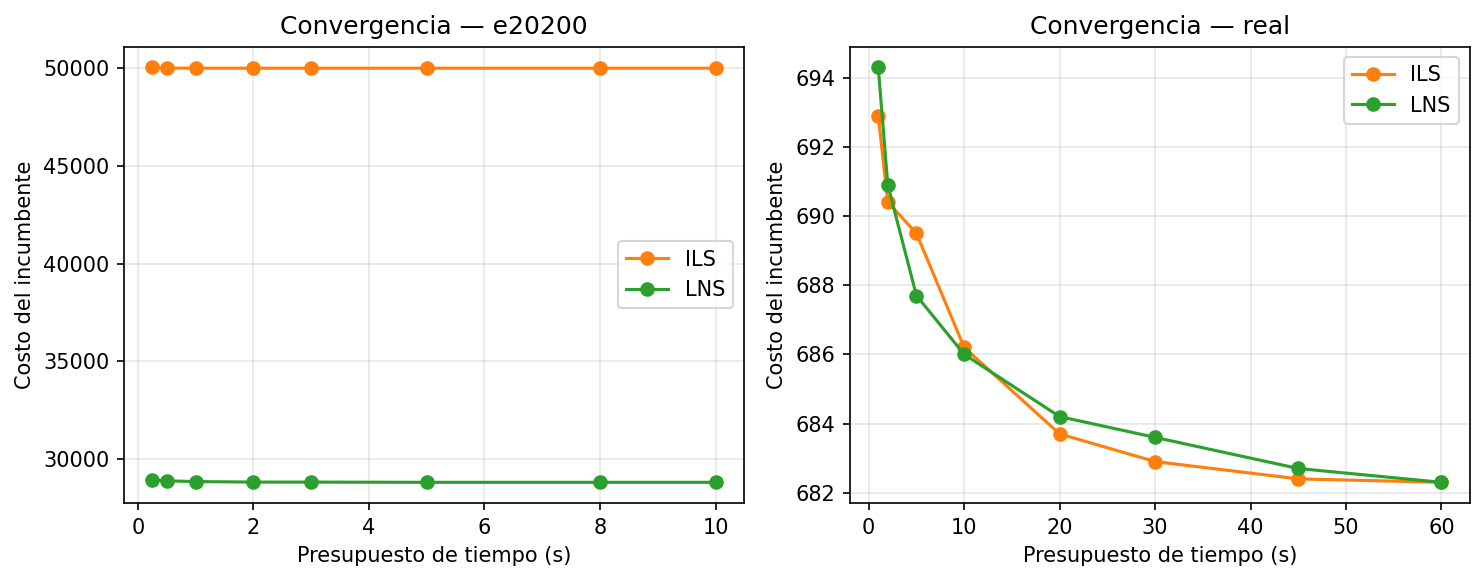
\includegraphics[width=0.92\linewidth]{figs/fig_convergencia.png}
\caption{Convergencia: costo del incumbente vs.\ presupuesto de tiempo, para ILS y LNS, en
una instancia ajustada (\code{e20200}) y en la real. LNS desciende más rápido en la
ajustada; en la real ambas convergen a valores similares.}
\label{fig:conv}
\end{figure}

\subsection{E5 --- Comparación final (RQ5)}
\emph{Hipótesis.} Esperábamos que la calidad creciera de forma monótona constructiva $<$ VND
$<$ metaheurística, con ganancias mayores en las instancias ajustadas, y que LNS marcara la
diferencia justamente ahí. La Tabla~\ref{tab:final} reporta el gap medio (\%) de cada método
respecto del mejor valor encontrado por instancia (menor es mejor), por grupo.

\begin{table}[ht]
\centering
\caption{Comparación final: gap medio (\%) respecto del mejor valor encontrado por instancia,
por método y grupo. Tiempo medio de la metaheurística (corte por tier). Menor gap es mejor.}
\label{tab:final}
\small
\begin{tabular}{l r r r r r}
\toprule
Grupo & Constructiva & VND & ILS & LNS & Tiempo MH (s) \\
\midrule
$a$ (prom.)   & 0,0  & 0,0  & 0,0  & \textbf{0,0} & 2,0 \\
$b$ (prom.)   & 26,4 & 17,8 & 14,0 & \textbf{0,0} & 2,0 \\
$e$ (prom.)   & 94,3 & 88,9 & 86,7 & \textbf{0,0} & 17,4 \\
\textbf{real} & 5,2  & 1,9  & 0,0  & \textbf{0,0} & 60,1 \\
\bottomrule
\end{tabular}
\end{table}

El detalle por semilla (Tabla~\ref{tab:ils_lns}) confirma el patrón: en las ajustadas ($b$, $e$)
LNS baja el costo medio muy por debajo de ILS (con más varianza, como en \code{e15900}); en la
holgada \code{a05100} y en la real ambas empatan.

\begin{table}[ht]
\centering
\caption{ILS vs.\ LNS: costo sobre 5 semillas (mejor / peor / medio / desvío) en una instancia
por grupo más la real. Menor es mejor; mejor costo medio por fila en negrita.}
\label{tab:ils_lns}
\small
\resizebox{\textwidth}{!}{%
\begin{tabular}{l r r r r r r r r}
\toprule
 & \multicolumn{4}{c}{ILS} & \multicolumn{4}{c}{LNS}\\
\cmidrule(lr){2-5}\cmidrule(lr){6-9}
Instancia & Mejor & Peor & Medio & Desvío & Mejor & Peor & Medio & Desvío \\
\midrule
a05100 & 1.694 & 1.694 & \textbf{1.694} & 0,00 & 1.694 & 1.694 & \textbf{1.694} & 0,00 \\
b10200 & 6.996 & 7.022 & 7.009,80 & 9,68 & 5.735 & 5.864 & \textbf{5.764,80} & 50,20 \\
e15900 & 617.375 & 617.389 & 617.383,20 & 5,38 & 351.670 & 423.046 & \textbf{387.206,20} & 27.002,29 \\
\textbf{real} & 682,30 & 684,80 & 683,56 & 0,95 & 682,30 & 683,70 & \textbf{682,90} & 0,52 \\
\bottomrule
\end{tabular}%
}
\end{table}

Se confirma la hipótesis: la progresión constructiva $\to$ VND $\to$ MH es monótona y LNS es el
mejor método en casi todo el \emph{benchmark} (gap $0\%$). ILS, atado a movimientos locales, no
reinserta los no asignados y su gap medio en $e$ llega a $86{,}7\%$; en el grupo $a$ y en la real
(holgados) todos convergen al mismo valor.

\begin{figure}[ht]
\begin{subfigure}{0.49\linewidth}
  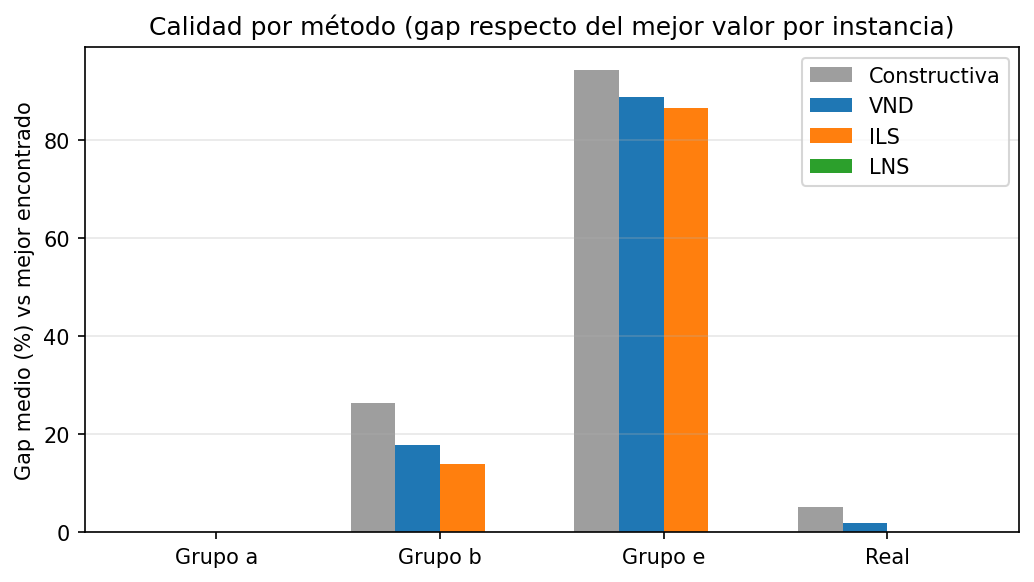
\includegraphics[width=\linewidth]{figs/fig_gap_metodo.png}
  \caption{Gap medio por método y grupo.}\label{fig:gap}
\end{subfigure}\hfill
\begin{subfigure}{0.49\linewidth}
  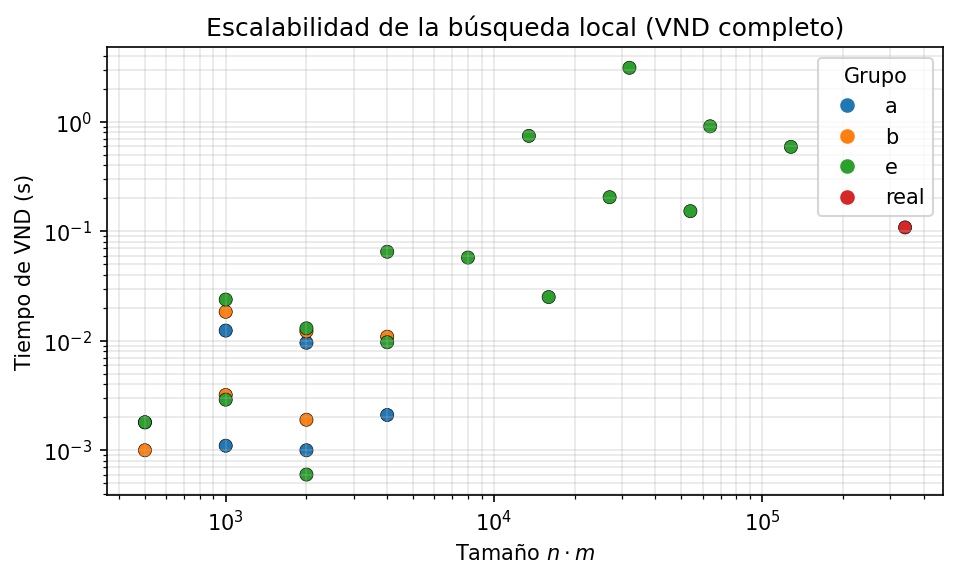
\includegraphics[width=\linewidth]{figs/fig_tiempo_tamano.png}
  \caption{Tiempo de VND vs.\ tamaño $n\cdot m$ (log-log).}\label{fig:tiempo}
\end{subfigure}
\caption{Resumen de la comparación final: calidad (gap) y escalabilidad de la búsqueda local.}
\end{figure}

\subsection{E6 --- Caso real ThunderPack (RQ6)}
\begin{table}[ht]
\centering
\caption{Instancia real ($m=310$, $n=1100$): costo, vendedores sin asignar, distancia media
por vendedor asignado y tiempo, por método (acumulado constructiva $\to$ VND $\to$ MH).}
\label{tab:real}
\small
\begin{tabular}{l r r r r}
\toprule
Método & Costo & Sin asignar & Distancia media & Tiempo (s) \\
\midrule
Mejor constructiva & 718,0 & 0 & 0,65 & $<0{,}01$ \\
+ VND              & 695,5 & 0 & 0,63 & 0,10 \\
+ ILS              & \textbf{682,3} & 0 & 0,62 & 60,1 \\
+ LNS              & \textbf{682,3} & 0 & 0,62 & 60,2 \\
\bottomrule
\end{tabular}
\end{table}

\begin{figure}[ht]
\centering
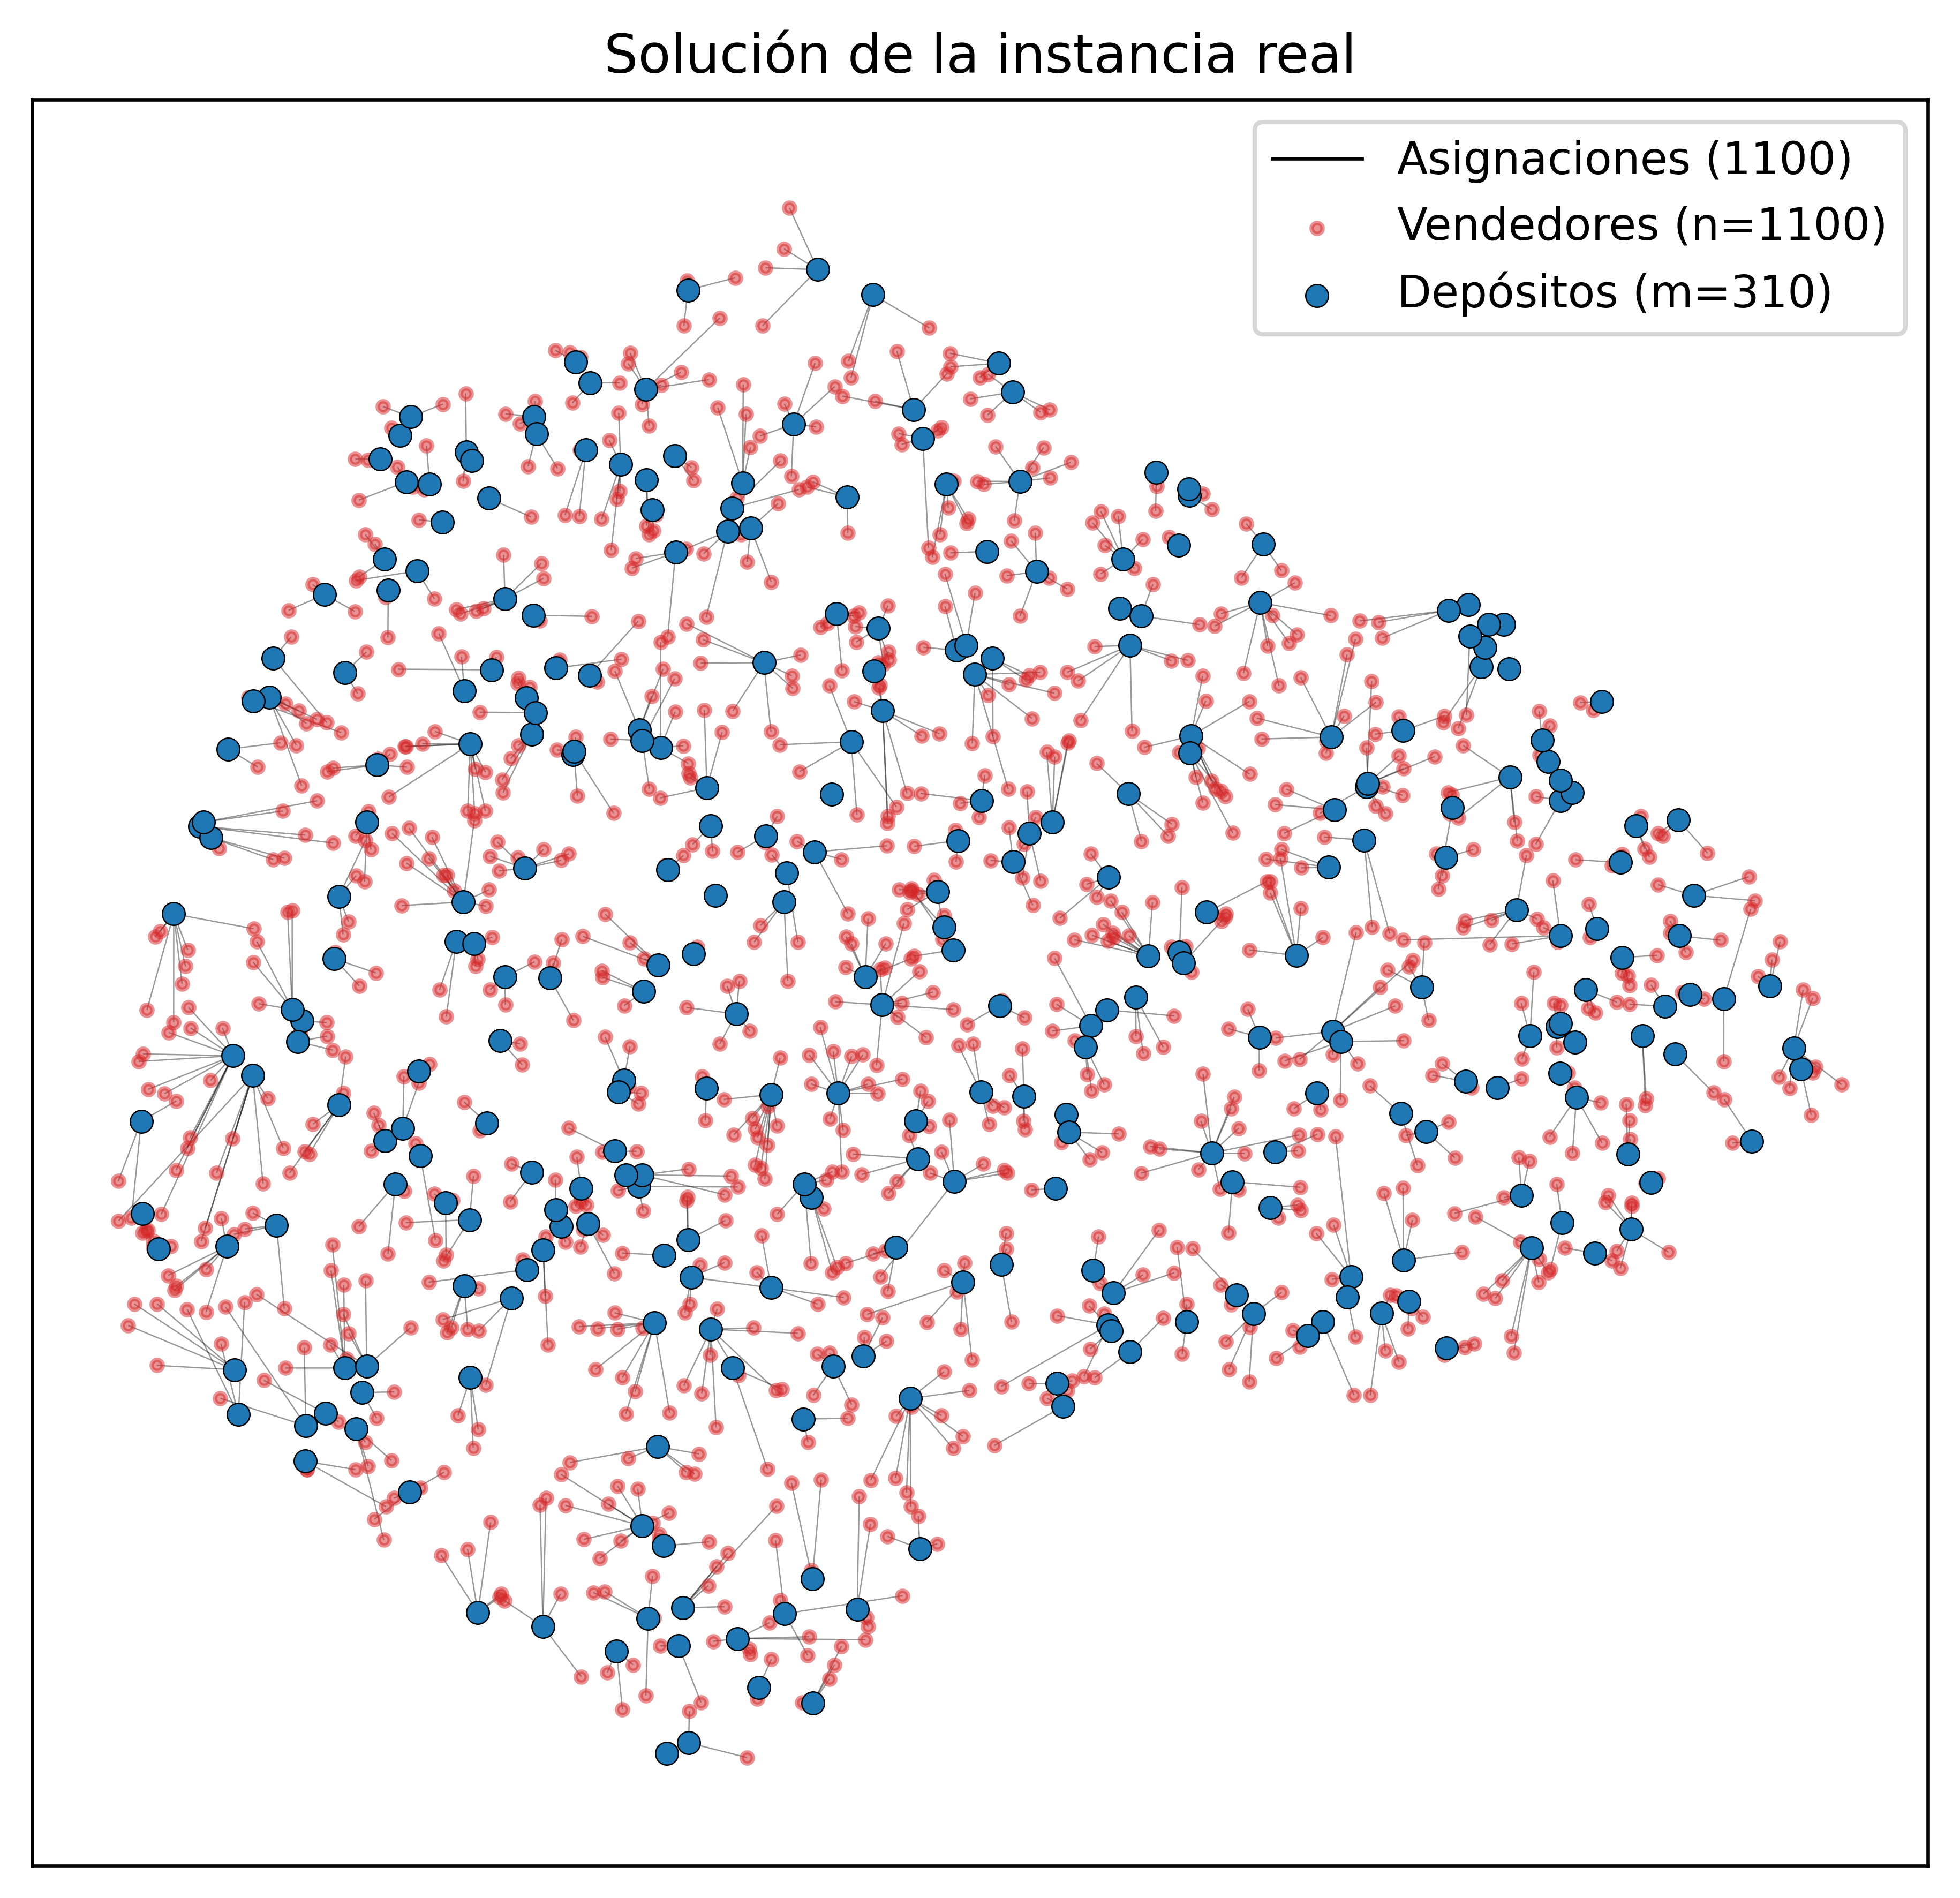
\includegraphics[width=0.55\linewidth]{figs/fig_mapa_real.png}
\caption{Disposición geográfica de la instancia real ($n=1100$ vendedores en rojo,
$m=310$ depósitos en azul; datos de \code{real\_instance.json}). Las líneas grises unen cada
vendedor con el depósito al que fue asignado en la solución de ILS (leída de \code{solucion\_competencia.txt}).}
\label{fig:mapa}
\end{figure}

\paragraph{Lectura de negocio (P1--P3).} La instancia real se resuelve con 0 vendedores sin
asignar por todos los métodos: la capacidad agregada (ratio $0{,}70$) alcanza y la geografía no
lo impide, así que la red no necesita ampliarse para la demanda actual (\textbf{P1}). La
distancia media por vendedor baja de $0{,}65$ (constructiva) a $0{,}62$ (con ILS/LNS), o sea
asignaciones cercanas y razonables (\textbf{P2}). En tiempo (\textbf{P3}), la constructiva es
instantánea, el VND tarda $\sim0{,}1$\,s y ya recorta $\sim3\%$, y las metaheurísticas en
$60$\,s ganan otro $\sim2\%$. En menos de un minuto se obtiene una solución de buena calidad,
viable como herramienta interactiva durante picos de demanda.

\subsection{E7 --- Peor y mejor caso (instancias sintéticas)}
Para ver en qué casos cada método falla o acierta, además del \emph{benchmark} construimos
instancias mínimas \emph{ad-hoc} (generadas dentro del archivo de \emph{testing}) que disparan
el peor y el mejor caso de cada tipo de método. La Tabla~\ref{tab:sinteticas} resume lo
observado.

\begin{table}[ht]
\centering
\caption{Peor/mejor caso sobre instancias sintéticas. En cada caso, el costo que obtiene
cada método sobre la misma instancia.}
\label{tab:sinteticas}
\small
\begin{tabular}{@{}l l r l@{}}
\toprule
Caso & Método & Costo & Interpretación \\
\midrule
\multirow{2}{*}{Greedy miope}
  & Vecino más cercano & 101 & \emph{peor caso} del greedy \\
  & Inserción (regret) & 3   & \emph{mejor caso} del regret \\
\midrule
\multirow{2}{*}{Óptimo local de 3 ciclos}
  & relocate + swap múltiples & 30 & atascado (\emph{peor caso} de 2 depósitos) \\
  & VND completo (ciclo3) & 3 & escapa (\emph{mejor caso} VND) \\
\midrule
\multirow{2}{*}{Metaheurística}
  & ILS desde mala constructiva & 3 & recupera el óptimo (\emph{mejor caso}) \\
  & ILS sobre instancia óptima & 2 & sin mejora: solo \emph{overhead} (\emph{peor caso}) \\
\bottomrule
\end{tabular}
\end{table}

En el caso \emph{greedy miope}, el vecino más cercano asigna el primer vendedor a un depósito
que el segundo necesitaba y queda en $101$, mientras que el regret resuelve en $3$. En el
\emph{óptimo local de 3 ciclos} se arma una asignación de la que ningún \emph{relocate múltiple}
ni \emph{swap múltiple} (de dos depósitos) puede salir, pero el \emph{cyclic exchange} de $3$ del
VND sí, y
eso justifica ese operador. Por último, la metaheurística recupera el óptimo desde una
constructiva muy mala, pero sobre una instancia ya óptima no puede mejorar: lo que gana depende
de cuánto margen deje la búsqueda local.

%==============================================================================
\section{Conclusiones, mejoras y observaciones}\label{sec:concl}
%==============================================================================
\begin{itemize}
  \item \textbf{Respuesta a P1--P3 (caso real).} La red actual alcanza (0 sin asignar, no hace
        falta ampliarla, \textbf{P1}), con distancias cercanas (media $0{,}65\to0{,}62$,
        \textbf{P2}) y solución en menos de un minuto (\textbf{P3}); detalle en E6
        (Tabla~\ref{tab:real}). En los grupos ajustados $b$/$e$ la lectura $d_j$ vuelve
        infactible asignar a todos.
  \item \textbf{ILS vs.\ LNS (hallazgo principal).} En instancias ajustadas LNS le gana a ILS
        por amplio margen, porque su destrucción-reconstrucción reubica vendedores no asignados
        que los movimientos locales de ILS no alcanzan; en la real (holgada) empatan.
        Recomendamos LNS por defecto, o un híbrido ILS+LNS.
  \item \textbf{Mejoras propuestas.} Criterio de aceptación tipo \emph{simulated annealing};
        \code{destruir} adaptativo en LNS; hibridar ILS+LNS; y generalizar el modelo a $d_{ij}$
        para comparar con los óptimos publicados.
  \item \textbf{Observaciones.} El \emph{regret} no domina siempre (empeora en $b$/$e$ bajo
        $d_j$); \emph{relocate múltiple} no aporta sobre estas constructivas (todo el trabajo lo
        hacen \emph{swap múltiple} y el \emph{ciclo de 3}); y la brecha
        constructiva--metaheurística crece con
        lo ajustada que sea la instancia.
\end{itemize}

%==============================================================================
\section{Solución entregada a la competencia}
%==============================================================================
Para la competencia corrimos el \emph{pipeline} completo (mejor constructiva $\to$ VND $\to$
metaheurística) sobre la instancia real de ThunderPack, dejándolo correr con un presupuesto de
\textbf{una hora}. La mejor solución obtenida tiene \textbf{costo $681{,}1$} (la distancia total
recorrida por los $1100$ vendedores), con \textbf{$0$ vendedores sin asignar} y una distancia
media de $\approx\!0{,}62$ por vendedor. La asignación completa se entrega en el archivo
\code{src/solucion\_competencia.txt}: una línea por depósito con los identificadores de los
vendedores asignados a ese depósito, en el formato del enunciado.

\end{document}
